\section{Stream Processing Architecture}\label{sec:concepts}
% Describe different ideas for distribution of events on multiple threads/processing and machines.
We have designed a data stream processing architecture based on the event producers and consumers concept that can be used to distribute the processing tasks to multiple threads (on a single machine), or separated processes (distribution on many commodity machines), or a combination of both.
Figure \ref{fig:parallel-srream-processing1} depicts our system architecture. The producers read the data stream batches from the remote network API (provided by DEBS2022 Challenge \cite{debs2022challenge}), and store them in a buffer queue in main memory.
The buffer queue has a specific size limitation that can be configured based on the available machine's RAM. The producer will read the data batches and store them in the queue until the queue size reaches the specific limit. Once the queue size is reached, the producer thread or process is suspended until the queue is available again to receive data.

The processing consumers access batches from the queue and process the events for Query 1 (values of $EMA_{38}$ and $EMA_{100}$)
and the subsequent Query 2. For the computation of $EMAs$, each consumer is required to know about the last $EMA$ value of the previous batch for a given stock symbol.
These consumer processes are the major query processing units that we call consumers for the sake of simplicity in this paper.

\begin{figure*}[!ht]
    \begin{center}
        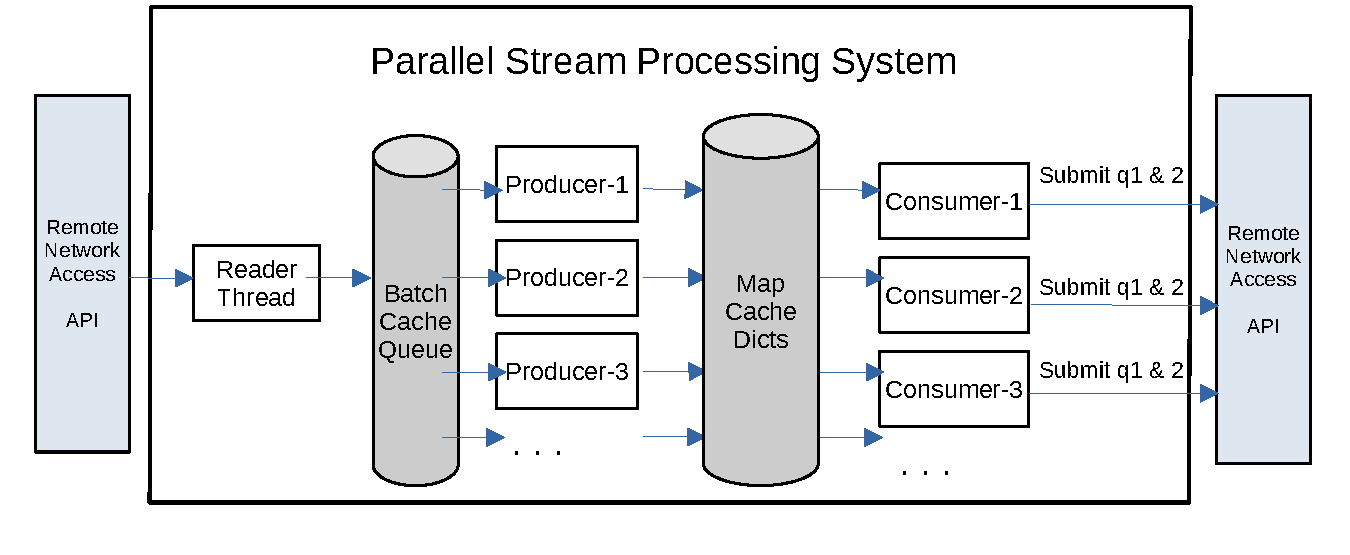
\includegraphics[width=0.7\textwidth]{./images/Parallel-Stream-Processing-System_v2}
        \caption{Parallel Processing of Events By a Set of Producers and Consumers without a Data Dispatcher.}
        \label{fig:parallel-srream-processing1}
    \end{center}
\end{figure*}

To make sure that there is no single bottleneck and synchronization lock point in this processing architecture, we made each of the consumers
(processing units) be responsible for monitoring and the computation of a sub-set of stocks symbol. Each consumer accesses the stream batches from the main memory cache and processes only the symbols that this consumer is responsible for them. This can be implemented by using hash functions on stock symbol and mapping it to the unique identification number of the consumer.
In our implementation, the hashing and distribution of the symbols to the consumers is processed in parallel by the producers.

Each consumer has a hash table that it uses to memoize the previous values of moving averages for different stock symbols.
In order to optimize for memory and time complexity, the only data stored per symbol include: the latest event (closing price) for the current window, the $EMA_{38}$ and $EMA_{100}$ of the previous window, and the last three crossover events.
Each consumer has to access events of each batch, and compute those stock symbols that the consumer is responsible for. With this approach, each consumer can work independently of any other consumers in a functional form. Access to each data batch from the queue should be implemented in an efficient manner so that each consumer does not read the entire batch to filter out the stock symbols it is responsible for.

Figures \ref{fig:parallel-srream-processing} and \ref{fig:batch-distributions} illustrate the system design if we have included an event dispatcher and an event submitter. We do not have a dispatcher and submitter because of efficiency reasons and because of the correctness of query processing.
If we dispatch the event batches as shown in Figure \ref{fig:parallel-srream-processing}, for example, by round-robin batch distribution, then each consumer has to work on all stock symbols or a subset of them.

If consumers work on all of the events, then each consumer required to know the previous moving averages from the immediate past batch to compute the new EMAs for the current data batch: implying a strict dependence on the preceding consumer before the current consumer can proceed.
This issue would cause incorrect processing, because a consumer should work in parallel distributed design, without any dependencies on each other's results.
In the former case, if the consumers work on a subset of stocks, we would need to pass every batch to all of the consumers, and it is better to do this task in an integrated form with reading from the queue.



\begin{figure*}[]
    \begin{center}
        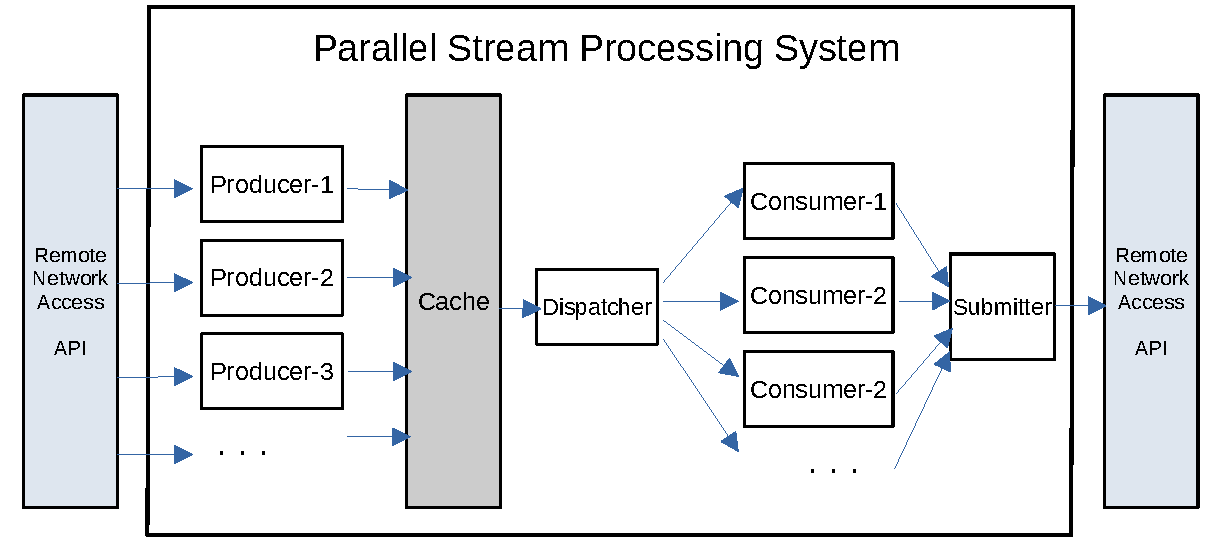
\includegraphics[width=0.7\textwidth]{./images/Parallel-Stream-Processing-System}
        \caption{Avoid Having a Event Dispatcher and Submitter.}
        \label{fig:parallel-srream-processing}
    \end{center}
\end{figure*}


\begin{figure*}[]
    \begin{center}
        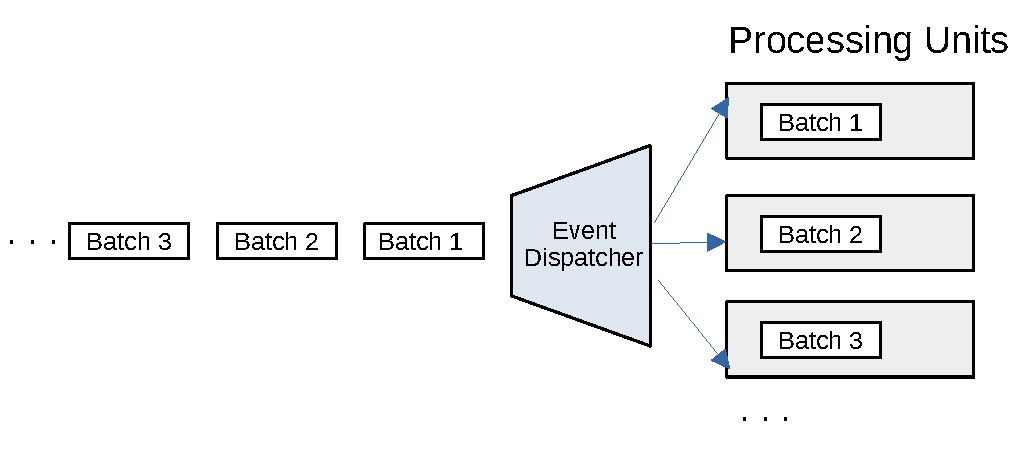
\includegraphics[width=0.7\textwidth]{./images/Stream-Batch-Distributions}
        \caption{An Event Data Dispatcher (Avoiding having a Dispatcher)}
        \label{fig:batch-distributions}
    \end{center}
\end{figure*}

Figure \ref{fig:Sequential-batch-distributions} illustrates how sequential data stream processing can work to process the batches in multiple
serial event consumers. Each processing unit will pick up and process a subset of stock market events.
In a single machine setup, the overhead of passing the event batches to the next consumer is very small, but in a distributed setting, the
overhead of passing data batches to the next consumer over the network is very high because of data serialization costs. Comparing the
architecture of Figure \ref{fig:Sequential-batch-distributions} and \ref{fig:parallel-srream-processing}, we preferred to implement the system
parallel format shown in Figure \ref{fig:parallel-srream-processing}.

\begin{figure*}[]
    \begin{center}
        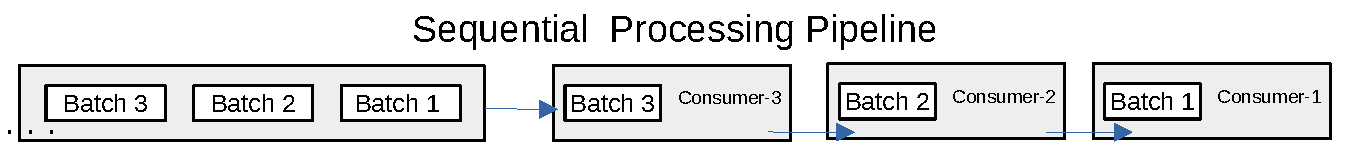
\includegraphics[width=0.7\textwidth]{./images/Stream-Batch-Distributions_op2}
        \caption{A Sequential Processing Pipeline. Each consumer reads a batch and passes to the next consumer. }
        \label{fig:Sequential-batch-distributions}
    \end{center}
\end{figure*}

The stream processing system will terminate if the stream of data is terminated, producers can not generate more event batches
and there is no event batch in the buffer queue.


%%%%%%%%%%%%%%%%%%%%%%%%%%%%%%%%%%%%%%%%%%%%%%%%%%%%%%%%
%%%%%%%%%%%%%%%%%%%%%%%%%%%%%%%%%%%%%%%%%%%%%%%%%%%%%%%%
%%%%%%%%%%    Implementation Details %%%%%%%%%%%%%%%%%%%
%%%%%%%%%%%%%%%%%%%%%%%%%%%%%%%%%%%%%%%%%%%%%%%%%%%%%%%%
%%%%%%%%%%%%%%%%%%%%%%%%%%%%%%%%%%%%%%%%%%%%%%%%%%%%%%%%



\section{Implementation Details}\label{sec:implementation}
The described architecture can be implemented using multiple threads on a single machine with multiple CPUs or distributed over a cluster of machines each with multiple CPU cores. Our first rapid alpha implementation of the system is in multi-threaded python code to make sure that we understand the challenge tasks and are able to process the queries in the correct form.


We realized that the processing task of Query 2 is a very simple computation that can be integrated with the Query 1 task.
The Listing \ref{lst:query2} provides a simple Python function that we use to check if we have a match for a breakout pattern.
This code can detect the breakouts (Crossover points) shown in Figure \ref{fig:EMAs}.
% Discuss the details of implementation.
% Add code how we do the Query 2.




\begin{minipage}{0.9\linewidth}
\begin{lstlisting}[caption={The computation for Query 2 - Breakout Patterns of EMA38 and EMA100}, label={lst:query2},language=Python]
def get_crossover(
    ema_38: float,
    ema_100: float,
    cur_38: float,
    cur_100: float,
    e: ch.Event
) -> Optional[ch.CrossoverEvent]:
""" Helper function for determining crossovers.
Args:
    ema_38 (float): The previous EMA38 value.
    ema_100 (float): The previous EMA100 value.
    cur_38 (float): The current EMA38 value.
    cur_100 (float): The current EMA100 value.
    e (ch.Event): Event.
Returns:
    Optional[ch.Crossover]: A crossover event.
"""
type = None
if ema_38 <= ema_100 and cur_38 > cur_100:
    type = ch.CrossoverEvent.SignalType.Buy
elif ema_38 >= ema_100 and cur_38 < cur_100:
    type = ch.CrossoverEvent.SignalType.Sell

if type is not None and e is not None:
    return ch.CrossoverEvent(
            ts=e.last_trade,
            symbol=e.symbol,
            security_type=e.security_type,
            signal_type=type
        )
return None
\end{lstlisting}
\end{minipage}





% \begin{minipage}{0.9\linewidth}
% \begin{lstlisting}[caption={Stream Processing Batch}, label={lst:createDataFrame4},language=Python]
% class ProcessBatches (threading.Thread):
% """ Producer thread to process batches. """
% def __init__(
%     self,
%     benchmark: Benchmark,
%     counter: Counter,
%     queue: Queue,
%     start_time: int,
%     num_consumers: int
% ) -> None:
%     """ Initializes the producer thread.
%     Args:
%         benchmark (Benchmark): Benchmark to submit to.
%         counter (Counter): Counter to synchronize pushing of batches.
%         queue (Queue): Queue to push batches to.
%         start_time (int): Reference start time.
%         num_consumers (int): Number of consumers.
%     """
%     threading.Thread.__init__(self)
%     self.benchmark = benchmark
%     self.counter = counter
%     self.queue = queue
%     self.start_time = start_time
%     self.num_consumers = num_consumers

% def run(self):
%     """ Processes batches by pushing onto the queue. """

%     while self.benchmark.has_next():
%         batch = self.benchmark.next()
%         obj = split_batch(batch, self.num_consumers, self.start_time)

%         # wait for counter to equal batch num
%         while not self.counter.is_value(obj[2]):
%             pass

%         # at this point counter == batch_num
%         self.queue.put(obj, block=True)

%         # increment counter so next batch can be put into the queue
%         self.counter.increment()
% \end{lstlisting}
% \end{minipage}

\textbf{Distributed Cluster Implementation.}\\
The architecture in Figure \ref{fig:parallel-srream-processing} can be implemented on a cluster of machines. The cache to store the stream batches can be implemented using shared memory on a single machine or using a service bus like Apache Kafka\footnote{\url{https://kafka.apache.org/}} or Apache Camel \footnote{\url{https://camel.apache.org/}} to store
the events and let multiple consumer clients access the streaming data batches.

Each consumer can subscribe to the event bus (e.g., Kafka) and receive only those stock prices that the specific consumer is responsible
for them. In this way, there will no dependencies between the consumers and there is no need to pass over the data batches to the next
consumer, also each consumer can submit the query result to the output sink.

One other implementation detail is to use a high-efficient data model and serialization framework for the data transmission between
the processing nodes. Studies have shown that choosing the correct data model and serialization have a huge impact on data processing performance \cite{DBLP:conf/cloud/SikdarTJ17}.

We suggest implementing the proposed architectural solution in a system programming language like C++ or Rust because of the statically typed variables and manually managed memory without an overhead of automated garbage collection. As described in Section \ref{sec:concepts}, the proposed architecture can be implemented using multiple threads on a single machine with multiple CPUs or distributed over a cluster of machines each with multiple CPU cores.
Our first rapid alpha implementation of the system is in multi-threaded Python code to make sure that we understand the challenge tasks and be able to process the queries in the correct form.
